\documentclass[letterpaper]{article}
\usepackage{listings}
\usepackage{booktabs}
\usepackage{array}
\usepackage{multirow}
\usepackage{amsmath,amssymb}
\usepackage{hhline}
\usepackage{authblk}
\usepackage[T1]{fontenc}
\usepackage{lipsum}
\usepackage{float}  
\usepackage{graphicx}
\usepackage[export]{adjustbox}
\usepackage{caption}
\usepackage{subcaption}
\usepackage[final]{pdfpages}
\usepackage{wrapfig}
\renewcommand{\baselinestretch}{2}

\usepackage[letterpaper, margin=1in]{geometry}

\begin{document}

\title{Train Controller User Manual}
\author{Written by: Andrew Lendacky}
\date{}

\maketitle


\section{Train Controller}

\subsection{UI Layout}

\begin{figure}[h!]
	\center
	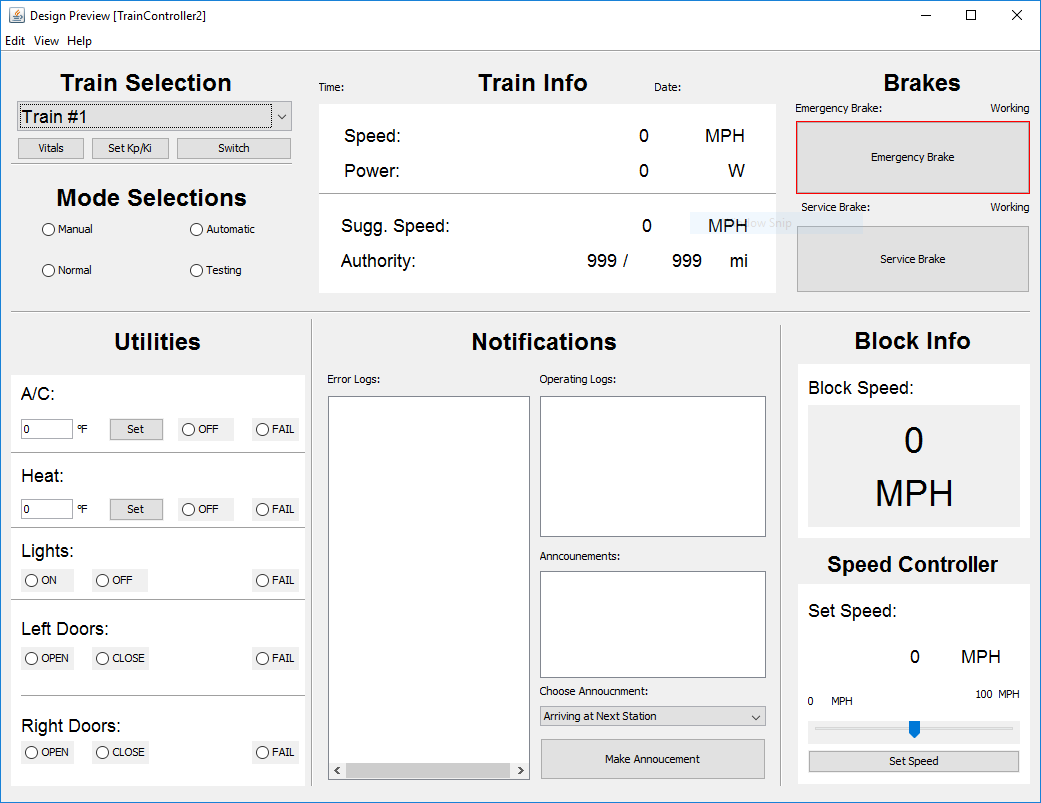
\includegraphics[width=16cm]{traincontroller_gui.PNG}
	\caption{Graphical User Interface for the train controller.}
\end{figure}

\begin{figure}[h!]
	\center
	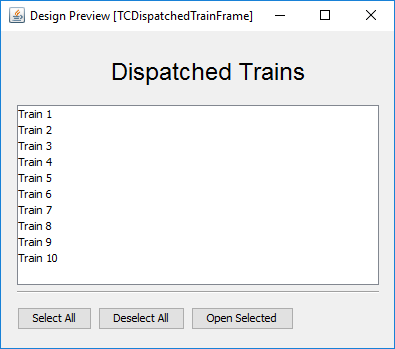
\includegraphics[width=10cm]{traincontroller_dispatchedtrains.PNG}
	\caption{User Interface for the dispatched trains.}
\end{figure}

\begin{figure}[h!]
	\center
	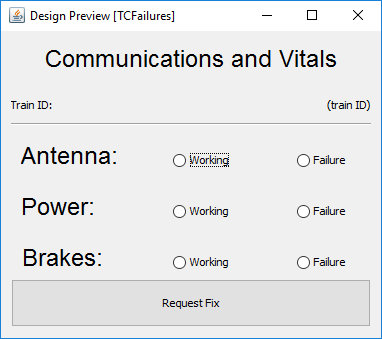
\includegraphics[width=10cm]{traincontroller_failurepanel.PNG}
	\caption{User interface for monitoring the failures of a train.}
\end{figure}

\begin{figure}[h!]
	\center
	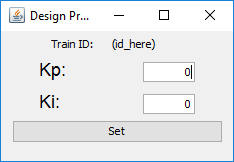
\includegraphics[width=10cm]{traincontroller_engineerpanel.PNG}
	\caption{User Interface for setting $K_p$ and $K_i$.}
\end{figure}

\subsection{UI Buttons and Actions}

	\subsubsection{Train Selection}
		\begin{itemize}
			\item Train Selection Dropdown - Clicking on the dropdown will allow the user to select a dispatched train.
			\item Switch - Clicking on this button will change the controls of this Train Controller to that of the selected train. 
			\item Vitals - Clicking on this button opens the Failures window (Figure 3) to monitor the status of the 3 failures that can occur on the train. If any failures exist, the button will be red.
			\item Set $K_p$/$K_i$ - Allows the user to control the power constants, $K_p$ and $K_i$. Clicking on this opens up Engineering Panel (Figure 4).
		\end{itemize}
	\subsubsection{Brake Controls}
	The operating status of both the emergency and service brakes can be seen above their respective button.
		\begin{itemize}
			\item Emergency Brake Button - Clicking on this button will open a window to confirm if you want to initiate the emergency brakes of the selected train. Clicking 'confirm' will apply the emergency brakes.
			\item Service Brake Button -  Clicking on this button will initiate the service brakes of the selected train.
		\end{itemize}
	
	\subsubsection{Speed Controller}
		\begin{itemize}
			\item Speed Slider - This slider controls setting the speed of the selected train. The max value of this slider is the max speed the train is allowed to go. In manual mode the max speed is determined by the block speed, and in automatic mode, the max speed is the suggested speed determined by the CTC.
			\item Set Speed Button - Clicking this button sends the selected speed to the train. 
		\end{itemize}
	\subsubsection{Block Information}
		\begin{itemize}
			\item Block Speed - This label displays the max speed of the block the selected train is in (miles per hour).  
		\end{itemize}
	\subsubsection{Train Information}
		\begin{itemize}
			\item Speed - Displays the speed the selected train is going (miles per hour). 
			\item Power - Displays the power the selected train is producing (watts). 
			\item Suggested Speed - Displays the speed that was suggested by the dispatcher (miles per hour). 
			\item Authority - Displays the authority that was set by the dispatcher and how much distance has elapsed (in miles).
		\end{itemize}
	\subsubsection{Mode Selections}
		\begin{itemize}
			\item Auto and Manual - Lets the user switch between Manual and Automatic mode. 
				\begin {itemize}
					\item Manual - The user controls the states of the selected train's Utilities (ON, OFF, OPEN, CLOSED, FAIL), controls the speed and initiates both brakes, as well as request repairs for any failures. 
					\item Automatic - The user cannot control the states of the selected train's Utilities (ON, OFF, OPEN, CLOSED, FAIL), the speed, repair requests, and the service brake. The user can only control the emergency brakes.
				\end{itemize}
			\item Normal and Testing - Lets the user switch between Normal and Testing mode. 
				\begin {itemize}
					\item Normal - The train controller operates cooperatively with all modules in the system. 
					\item Testing - Opens a window that allows the user to operate the Train Controller without the other necessary modules. 
				\end{itemize}
		\end{itemize}
	\subsubsection{Notifcations}
		\begin{itemize}
			\item Error Logs - Displays any errors or failures that the selected train has or had and at what time.
			\item Operating Logs - Displays operating logs about selected train.
			\item Announcements - Displays any previously made announcements to the screen and at what time. 
			\item Choose Announcement Dropdown - If in manual mode, lets the user pick from a list of available announcements to make. 
			\item Make Announcement Button - Transmits the selected announcement from the announcement dropdown through the train's speaker system. 
		\end{itemize}
	\subsubsection{Utilities}
	Manual Mode: The driver can change the state of these utilities as well as set the desired temperature of the air conditioning and heating unit. If any of the utilities are in the FAIL state, they must be fixed before the driver can change their state. Attempting to change the state while in FAIL will result in a error window. To request a fix, go to View > Failures from the menu bar or click 'Vitals' under the train selection dropdown.
	\newline
	Automatic Mode: The user cannot control the states of these buttons, and are set according to the instruments (thermostat, light sensor, etc..) on the train. The status of these buttons will be selected based on the states of utilities on the selected train.
		\begin{itemize}
			\item Air Conditioning (AC) - Controls and displays the state of the AC unit on the selected train. If in manual mode, the user can also set the temperature of the AC unit to a specific degree by typing it in the textfield and clicking SET. 
			\item Heat - Controls and display the state of the heating unit on the selected train. If in manual mode, the user can also set the temperature of the heating unit to a specific degree by typing it in the textfield and clicking SET.
			\item Lights - Controls the state (ON, OFF) of the Lights on the selected train. 
			\item Left and Right Doors - Controls and displays the states (OPEN, CLOSED) of the left and right doors of the selected train.  
		\end{itemize}
	
\subsection{Menu Bar and Popups}

The Train Controller includes a menu bar to help access and set specific information.  

\subsubsection{Edit}
	\begin{itemize}
		\item Set $K_{p}$ and $K_{i}$ - Allows the engineer to set $K_{p}$ and $K_{i}$ which is used to calculate the power needed to reach a certain speed. Clicking on the menu item will open up the Engineering Panel (Figure 4) where the user can set the $K_{p}$ and $K_{i}$ by typing them into the textfield and clicking SET.
		\item Open Train Controller - Opens a new Train Controller window. This allows for multiple trains to be controlled at once. 
	\end{itemize}

\subsubsection{View}
	\begin{itemize}
		\item Dispatched Trains - Opens a window (Figure 2) with a list of all dispatched trains. The user can select multiple trains by holding down SHIFT on the keyboard. Clicking on the 'Open Selected' will open a Train Controller for each of the selected trains.  
		\item Failures - Opens the Failure Panel (Figure 3) which shows the status (Working/Failure) of the three failures that can occur on the train (power, antenna, and brake). If any of these failures exist, the user can request a fix by clicking on 'Request Fix'. 
	\end{itemize}
	 
\subsubsection{Help}
	\begin{itemize}
		\item View User Manual - Opens up the User Manual in PDF format in a new window. 
		\item Toggle Tooltips - Changes if the tooltips are enabled or not. Tooltips are on by default, and display relevant information about a given button on the GUI when hovering your mouse over it. Almost all elements on the Train Controller have a tooltip. 
		\item About - Displays a brief description about the Train Controller in a new window.
	\end{itemize}


\end{document}